\documentclass[lualatex,ja=standard,a4paper,12pt]{bxjsarticle}
\usepackage{amsmath, amssymb, amsthm}
\usepackage{geometry}
\usepackage{xcolor}
\usepackage{tcolorbox}
\usepackage{booktabs}
\usepackage{array}
\usepackage{pgfplots}
\pgfplotsset{compat=1.18}

\geometry{margin=25mm}
\tcbuselibrary{theorems, skins, breakable}

\newtcolorbox{defbox}[1]{
  colback=blue!5, colframe=blue!60!black,
  fonttitle=\bfseries, title={#1}, arc=3pt
}
\newtcolorbox{thmbox}[1]{
  colback=green!5, colframe=green!50!black,
  fonttitle=\bfseries, title={#1}, arc=3pt, breakable
}
\newtcolorbox{derivbox}[1]{
  colback=yellow!6, colframe=yellow!70!black,
  fonttitle=\bfseries, title={計算：#1}, arc=3pt, breakable
}
\newtcolorbox{pointbox}{
  colback=orange!8, colframe=orange!70!black,
  fonttitle=\bfseries, title={ポイント}, arc=3pt
}
\newtcolorbox{exbox}[1]{
  colback=gray!6, colframe=gray!50,
  fonttitle=\bfseries, title={例：#1}, arc=3pt, breakable
}

\newtheorem{theorem}{定理}
\newtheorem{proposition}[theorem]{命題}
\newtheorem{definition}[theorem]{定義}
\newtheorem{remark}[theorem]{注意}

\title{\textbf{変数変換と確率密度} \\[6pt]
       {\large 微分形式の視点から}}
\author{}
\date{}

\begin{document}
\maketitle
\thispagestyle{empty}
\tableofcontents
\newpage

%===========================================
\section{序：なぜ密度変換にヤコビアンが現れるのか}
%===========================================

確率密度関数 $f_X(x)$ は「確率そのもの」ではなく，
「単位長さあたりの確率」すなわち\textbf{密度}である．
確率はその密度を積分して得られる：
\[
  P(a \leq X \leq b) = \int_a^b f_X(x)\,dx.
\]
ここで $dx$ は「長さの要素」であり，$f_X(x)$ は「その長さ要素における密度」である．

$Y = g(X)$ と変換したとき，$f_Y$ を求める問題は本質的に
「$x$ 座標系の長さ要素 $dx$ が $y$ 座標系の長さ要素 $dy$ にどう対応するか」
という\textbf{座標変換の問題}である．

ヤコビアンはこの「長さ・面積・体積の変換比」を記述するものであり，
その本質は\textbf{微分形式（differential form）}の言語で最もエレガントに表現される．

%===========================================
\section{1次元の場合：微分と長さ要素}
%===========================================

\subsection{微分 $df$ と 1-形式}

滑らかな関数 $g: \mathbb{R} \to \mathbb{R}$ に対して，$y = g(x)$ の微分は
\[
  dy = g'(x)\,dx
\]
と書ける．これは「$x$ が $dx$ だけ動くと，$y$ は $g'(x)\,dx$ だけ動く」という情報を持つ．

$dx$ を「$x$ 軸上の（符号付き）長さの素」として捉えると，$dy = g'(x)\,dx$ は
$x$ 軸上の長さ要素が $y$ 軸上でどう変換されるかを表す式である．

\subsection{積分の変換と確率の保存}

$g$ が $[a,b]$ 上の微分同相（単調な滑らかな全単射）のとき，
\[
  \int_{g(a)}^{g(b)} h(y)\,dy = \int_a^b h(g(x))\,|g'(x)|\,dx.
\]

確率への応用：$P(a \leq X \leq b) = P(g(a) \leq Y \leq g(b))$ を使うと，
\begin{align*}
  \int_{g(a)}^{g(b)} f_Y(y)\,dy
  &= \int_a^b f_X(x)\,dx
   = \int_{g(a)}^{g(b)} f_X(g^{-1}(y)) \cdot \frac{1}{|g'(g^{-1}(y))|}\,dy.
\end{align*}

被積分関数を比較することで，

\begin{thmbox}{1次元の密度変換公式}
$Y = g(X)$，$g$ が微分同相のとき，
\[
  f_Y(y) = f_X(g^{-1}(y)) \cdot \left|\frac{d}{dy}g^{-1}(y)\right|
          = f_X(g^{-1}(y)) \cdot \frac{1}{|g'(g^{-1}(y))|}.
\]
\end{thmbox}

\begin{exbox}{$Y = 1/X$（逆ガンマ分布の導出）}
$g(x) = 1/x$，$g^{-1}(y) = 1/y$，$\frac{d}{dy}(1/y) = -1/y^2$．

したがって：
\[
  f_Y(y) = f_X(1/y) \cdot \frac{1}{y^2}.
\]
$X \sim \mathrm{Gamma}(a, b)$，すなわち $f_X(x) \propto x^{a-1}e^{-bx}$ とすると，
\[
  f_Y(y) \propto (1/y)^{a-1} e^{-b/y} \cdot y^{-2} = y^{-a-1} e^{-b/y}.
\]
これが逆ガンマ分布の密度である．
\end{exbox}

%===========================================
\section{多次元の場合：ヤコビアン行列}
%===========================================

\subsection{線形写像と面積の変換}

$\mathbb{R}^2$ の線形写像 $A : \mathbb{R}^2 \to \mathbb{R}^2$ を考える．
単位正方形 $[0,1]^2$ の面積は $1$ であるが，$A$ で写すと平行四辺形になる．
この平行四辺形の面積は $|\det A|$ に等しい．

\begin{center}
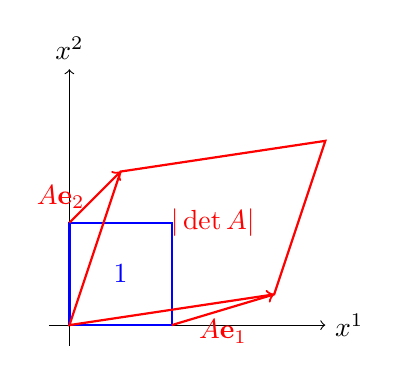
\begin{tikzpicture}[scale=1.3]
  \draw[->] (-0.2,0) -- (2.5,0) node[right] {$x^1$};
  \draw[->] (0,-0.2) -- (0,2.5) node[above] {$x^2$};
  % original square
  \draw[blue, thick] (0,0) -- (1,0) -- (1,1) -- (0,1) -- cycle;
  \node[blue] at (0.5, 0.5) {$1$};
  % transformed parallelogram (A = [[2,0.5],[0.3,1.5]])
  \draw[red, thick] (0,0) -- (2,0.3) -- (2.5,1.8) -- (0.5,1.5) -- cycle;
  \node[red] at (1.4, 1.0) {$|\det A|$};
  \draw[red, ->, thick] (1,0) -- (2,0.3) node[midway, below] {$A\mathbf{e}_1$};
  \draw[red, ->, thick] (0,1) -- (0.5,1.5) node[midway, left] {$A\mathbf{e}_2$};
\end{tikzpicture}
\end{center}

一般に，行列式は「写像が単位体積をどれだけ拡大・縮小するか」を表す：
\[
  \mathrm{Vol}(A(S)) = |\det A| \cdot \mathrm{Vol}(S).
\]

\subsection{ヤコビアン行列と多変数変換定理}

滑らかな写像 $\boldsymbol{\phi}: U \subset \mathbb{R}^n \to V \subset \mathbb{R}^n$，
$\mathbf{y} = \boldsymbol{\phi}(\mathbf{u})$ に対して，
\textbf{ヤコビアン行列}を
\[
  D\boldsymbol{\phi}(\mathbf{u})
  = \begin{pmatrix}
    \dfrac{\partial \phi^1}{\partial u^1} & \cdots & \dfrac{\partial \phi^1}{\partial u^n} \\[8pt]
    \vdots & \ddots & \vdots \\[4pt]
    \dfrac{\partial \phi^n}{\partial u^1} & \cdots & \dfrac{\partial \phi^n}{\partial u^n}
    \end{pmatrix}
\]
と定義する．$D\boldsymbol{\phi}(\mathbf{u})$ は点 $\mathbf{u}$ における $\boldsymbol{\phi}$ の「最良の線形近似」であり，
点 $\mathbf{u}$ の近傍での体積変換比は $|\det D\boldsymbol{\phi}(\mathbf{u})|$ で与えられる．

\begin{thmbox}{多変数の変換定理}
$\boldsymbol{\phi}: U \to V$ が微分同相，$h: V \to \mathbb{R}$ が可積分なとき，
\[
  \int_V h(\mathbf{y})\, d\mathbf{y}
  = \int_U h(\boldsymbol{\phi}(\mathbf{u}))\, |\det D\boldsymbol{\phi}(\mathbf{u})|\, d\mathbf{u}.
\]
\end{thmbox}

%===========================================
\section{微分形式：エレガントな定式化}
%===========================================

変数変換定理は，微分形式の言語を使うと「プルバック（pullback）」という
一つの操作として統一的に記述できる．

\subsection{$n$-形式と面積・体積要素}

$\mathbb{R}^2$ 上の\textbf{2-形式}（2-form）の典型例は
\[
  \omega = dx^1 \wedge dx^2
\]
であり，「$x^1$-$x^2$ 平面の符号付き面積要素」を表す抽象的なオブジェクトである．

ウェッジ積 $\wedge$ は\textbf{交代的（alternating）かつ双線型}な積で，特に
\[
  dx^i \wedge dx^j = -dx^j \wedge dx^i, \qquad dx^i \wedge dx^i = 0.
\]

一般に $\mathbb{R}^n$ の $n$-形式は $f(\mathbf{x})\,dx^1 \wedge \cdots \wedge dx^n$ の形をとり，
$\int_U f(\mathbf{x})\,dx^1 \wedge \cdots \wedge dx^n$ をルベーグ積分として定義する．

\subsection{プルバック（Pullback）}

写像 $\boldsymbol{\phi}: U \to V$ に対して，$V$ 上の微分形式 $\omega$ の
$U$ への\textbf{プルバック} $\boldsymbol{\phi}^*\omega$ を次のように定義する：

$\boldsymbol{\phi}$ によって $\mathbf{u} \mapsto \mathbf{y} = \boldsymbol{\phi}(\mathbf{u})$ と座標を変えるとき，
1-形式 $dy^i$ のプルバックは
\[
  \boldsymbol{\phi}^*(dy^i) = d\phi^i = \sum_j \frac{\partial \phi^i}{\partial u^j}\,du^j.
\]
つまり「$dy^i$ を $\boldsymbol{\phi}$ で引き戻す」とは，「$y^i = \phi^i(\mathbf{u})$ を全微分する」ことである．

$n$-形式への拡張はウェッジ積の多重線型性から従う：

\begin{thmbox}{$n$-形式のプルバック}
\[
  \boldsymbol{\phi}^*(dy^1 \wedge \cdots \wedge dy^n)
  = d\phi^1 \wedge \cdots \wedge d\phi^n
  = \det(D\boldsymbol{\phi})\; du^1 \wedge \cdots \wedge du^n.
\]
\end{thmbox}

\begin{derivbox}{ウェッジ積の交代性から行列式が出る理由}
$n=2$ で確認する．$\phi^1, \phi^2: U \to \mathbb{R}$ とすると，
\begin{align*}
  d\phi^1 \wedge d\phi^2
  &= \left(\frac{\partial \phi^1}{\partial u^1}du^1 + \frac{\partial \phi^1}{\partial u^2}du^2\right)
     \wedge
     \left(\frac{\partial \phi^2}{\partial u^1}du^1 + \frac{\partial \phi^2}{\partial u^2}du^2\right).
\end{align*}
ウェッジ積を展開する（$du^i \wedge du^i = 0$，$du^2 \wedge du^1 = -du^1 \wedge du^2$ を使う）：
\begin{align*}
  &= \frac{\partial \phi^1}{\partial u^1}\frac{\partial \phi^2}{\partial u^2}\,du^1\wedge du^2
   + \frac{\partial \phi^1}{\partial u^2}\frac{\partial \phi^2}{\partial u^1}\,du^2\wedge du^1 \\
  &= \left(
      \frac{\partial \phi^1}{\partial u^1}\frac{\partial \phi^2}{\partial u^2}
     -\frac{\partial \phi^1}{\partial u^2}\frac{\partial \phi^2}{\partial u^1}
     \right) du^1\wedge du^2 \\
  &= \det(D\boldsymbol{\phi})\; du^1\wedge du^2. \hspace{6cm}\square
\end{align*}
ウェッジ積の交代性（$du^2 \wedge du^1 = -du^1\wedge du^2$）が
\textbf{自動的に行列式の交代性を生み出している}．
これが微分形式の言語のエレガントさである．
\end{derivbox}

\subsection{変数変換定理の形式的表現}

プルバックを使うと，変数変換定理は
\[
  \int_V h\,\omega = \int_U \boldsymbol{\phi}^*(h\,\omega)
  = \int_U (h \circ \boldsymbol{\phi})\cdot\det(D\boldsymbol{\phi})\; du^1\wedge\cdots\wedge du^n
\]
と書ける（向きに注意して $|\det|$ とする）．

積分とは「$n$-形式を積分する操作」であり，
座標変換とは「$n$-形式を引き戻す操作（プルバック）」である．
この観点から，変数変換定理は
\[
  \boxed{\text{座標変換のもとで積分は不変}\;\Leftrightarrow\;
         \text{プルバックが体積要素の変換比（ヤコビアン）を自動的に補正する}}
\]
という命題に他ならない．

%===========================================
\section{極座標への応用}
%===========================================

\subsection{面積要素 $dA = r\,dr\,d\theta$ のプルバックによる導出}

極座標への変換 $\boldsymbol{\phi}: (r, \theta) \mapsto (x, y) = (r\cos\theta, r\sin\theta)$ を考える．

\begin{derivbox}{プルバック $\boldsymbol{\phi}^*(dx\wedge dy)$ の計算}
まず 1-形式の全微分を求める：
\begin{align*}
  dx &= d(r\cos\theta) = \cos\theta\,dr - r\sin\theta\,d\theta, \\
  dy &= d(r\sin\theta) = \sin\theta\,dr + r\cos\theta\,d\theta.
\end{align*}

ウェッジ積を計算する：
\begin{align*}
  dx\wedge dy
  &= (\cos\theta\,dr - r\sin\theta\,d\theta)
     \wedge(\sin\theta\,dr + r\cos\theta\,d\theta) \\
  &= \cos\theta\sin\theta\underbrace{dr\wedge dr}_{0}
   + r\cos^2\theta\,dr\wedge d\theta
   - r\sin^2\theta\,d\theta\wedge dr
   - r^2\sin\theta\cos\theta\underbrace{d\theta\wedge d\theta}_{0} \\
  &= r\cos^2\theta\,dr\wedge d\theta
   + r\sin^2\theta\,dr\wedge d\theta
   \quad (d\theta\wedge dr = -dr\wedge d\theta \text{ を使用}) \\
  &= r(\cos^2\theta + \sin^2\theta)\,dr\wedge d\theta
   = r\,dr\wedge d\theta.
\end{align*}
\end{derivbox}

したがって，
\[
  \boldsymbol{\phi}^*(dx\wedge dy) = r\,dr\wedge d\theta,
\]
すなわち面積要素 $dA = dx\,dy$ は極座標では $dA = r\,dr\,d\theta$ になる．
係数 $r$ がヤコビアンであり，$\det(D\boldsymbol{\phi}) = r$ に対応する：

\[
  D\boldsymbol{\phi} =
  \begin{pmatrix}
    \partial x/\partial r & \partial x/\partial\theta \\
    \partial y/\partial r & \partial y/\partial\theta
  \end{pmatrix}
  =
  \begin{pmatrix} \cos\theta & -r\sin\theta \\ \sin\theta & r\cos\theta \end{pmatrix},
  \qquad
  \det(D\boldsymbol{\phi}) = r\cos^2\theta + r\sin^2\theta = r.
\]

\subsection{応用：ガウス積分 $\int_{-\infty}^{\infty} e^{-x^2/2}\,dx = \sqrt{2\pi}$}

\begin{derivbox}{ガウス積分の計算（極座標変換）}
$I = \int_{-\infty}^{\infty} e^{-x^2/2}\,dx$ とおく．$I^2$ を 2 次元積分で表す：
\[
  I^2 = \int_{\mathbb{R}^2} e^{-(x^2+y^2)/2}\,dx\wedge dy.
\]
極座標変換 $x = r\cos\theta$，$y = r\sin\theta$（$r>0$，$\theta\in[0,2\pi)$）を適用する．
プルバックにより $dx\wedge dy = r\,dr\wedge d\theta$ なので，
\begin{align*}
  I^2
  &= \int_0^{2\pi}\int_0^{\infty} e^{-r^2/2}\cdot r\,dr\,d\theta
   = 2\pi \int_0^{\infty} r\,e^{-r^2/2}\,dr.
\end{align*}
$u = r^2/2$，$du = r\,dr$ と置換すると：
\[
  I^2 = 2\pi\int_0^{\infty} e^{-u}\,du = 2\pi. \hspace{4cm}\square
\]
よって $I = \sqrt{2\pi}$，すなわち正規分布の規格化定数が確認できる．
\end{derivbox}

%===========================================
\section{確率密度への統一的応用}
%===========================================

\subsection{密度変換の一般公式}

$\mathbf{X}: \Omega \to \mathbb{R}^n$ が確率ベクトルで，$\mathbf{Y} = g(\mathbf{X})$（$g$ は微分同相）のとき，
$\boldsymbol{\phi} = g^{-1}$（逆写像）のプルバックを考えると：

\[
  P(\mathbf{Y} \in A)
  = P(\mathbf{X} \in g^{-1}(A))
  = \int_{g^{-1}(A)} f_{\mathbf{X}}(\mathbf{x})\,d\mathbf{x}
  = \int_A f_{\mathbf{X}}(g^{-1}(\mathbf{y}))\,|\det D g^{-1}(\mathbf{y})|\,d\mathbf{y}.
\]

\begin{thmbox}{多変数の密度変換公式}
\[
  f_{\mathbf{Y}}(\mathbf{y}) = f_{\mathbf{X}}(g^{-1}(\mathbf{y})) \cdot |\det D g^{-1}(\mathbf{y})|.
\]
ヤコビアン $|\det D g^{-1}|$ は「$\mathbf{y}$ 座標系の体積要素が $\mathbf{x}$ 座標系の体積要素の
何倍か」を表す補正因子である．
\end{thmbox}

\subsection{例：Box--Muller 変換（一様分布 $\to$ 正規分布）}

\begin{exbox}{Box--Muller 変換}
$U_1, U_2 \overset{\mathrm{i.i.d.}}{\sim} \mathrm{Uniform}(0,1)$ を独立な一様乱数とする．
\[
  Z_1 = \sqrt{-2\ln U_1}\cos(2\pi U_2), \qquad
  Z_2 = \sqrt{-2\ln U_1}\sin(2\pi U_2)
\]
と定義すると，$Z_1, Z_2$ は独立な標準正規変数になる．

\medskip
\noindent\textbf{確認：}

逆写像 $g^{-1}: (z_1, z_2) \mapsto (u_1, u_2)$ は
\[
  u_1 = e^{-(z_1^2+z_2^2)/2}, \qquad u_2 = \frac{1}{2\pi}\arctan\frac{z_2}{z_1}.
\]

ヤコビアン行列を計算する：
\[
  D g^{-1} =
  \begin{pmatrix}
    -z_1\,e^{-r^2/2} & -z_2\,e^{-r^2/2} \\[4pt]
    \dfrac{-z_2}{2\pi r^2} & \dfrac{z_1}{2\pi r^2}
  \end{pmatrix},
  \qquad r^2 = z_1^2 + z_2^2.
\]

行列式：
\begin{align*}
  \det D g^{-1}
  &= (-z_1 e^{-r^2/2})\cdot\frac{z_1}{2\pi r^2}
   - (-z_2 e^{-r^2/2})\cdot\frac{-z_2}{2\pi r^2} \\
  &= \frac{-e^{-r^2/2}}{2\pi r^2}(z_1^2 + z_2^2)
   = -\frac{e^{-r^2/2}}{2\pi}.
\end{align*}

$f_{U_1,U_2}(u_1,u_2) = 1$（一様分布）なので，
\begin{align*}
  f_{Z_1,Z_2}(z_1,z_2)
  &= 1 \cdot \left|\det D g^{-1}\right|
   = \frac{e^{-(z_1^2+z_2^2)/2}}{2\pi} \\
  &= \underbrace{\frac{1}{\sqrt{2\pi}}e^{-z_1^2/2}}_{Z_1 \sim N(0,1)}
     \cdot
     \underbrace{\frac{1}{\sqrt{2\pi}}e^{-z_2^2/2}}_{Z_2 \sim N(0,1)}.
\end{align*}
因数分解できているので $Z_1, Z_2$ は独立．
\noindent\textbf{この変換は「$(r, \theta)$ 極座標への変換」と本質的に同じ構造をしている．}
\end{exbox}

%===========================================
\section{Radon--Nikodym 微分との接続（発展）}
%===========================================

より抽象的な視点では，確率密度は\textbf{ルベーグ測度に対する Radon--Nikodym 微分}である．

$\mu_X$ を $X$ の確率測度，$\lambda$ をルベーグ測度とすると，
$f_X$ が存在するとは $\mu_X \ll \lambda$（絶対連続）であることを意味し，
\[
  f_X = \frac{d\mu_X}{d\lambda}.
\]

$Y = g(X)$ のとき，$\mu_Y$ は $\mu_X$ の「$g$ による押し出し測度（pushforward measure）」：
\[
  \mu_Y(A) = \mu_X(g^{-1}(A)).
\]

密度変換公式はこの押し出しを Radon--Nikodym の言語で書いたものである：
\[
  \frac{d\mu_Y}{d\lambda}(\mathbf{y})
  = \frac{d\mu_X}{d\lambda}(g^{-1}(\mathbf{y})) \cdot \left|\det D g^{-1}(\mathbf{y})\right|.
\]

ヤコビアン $|\det D g^{-1}|$ は「ルベーグ測度を $g$ で押し出した測度と元のルベーグ測度の比」，
すなわちルベーグ測度同士の Radon--Nikodym 微分
\[
  \left|\det D g^{-1}(\mathbf{y})\right| = \frac{d(g_*\lambda)}{d\lambda}(\mathbf{y})
\]
に他ならない．

\begin{pointbox}
\textbf{まとめ：三つの視点}
\begin{center}
\renewcommand{\arraystretch}{1.5}
\begin{tabular}{lp{9cm}}
\toprule
\textbf{視点} & \textbf{ヤコビアンの意味} \\
\midrule
初等的（確率の保存） &
  小区間・小領域の確率を等しくするための補正因子 \\
微分形式 &
  $n$-形式のプルバック $\boldsymbol{\phi}^*(d\mathbf{x}) = |\det D\boldsymbol{\phi}|\,d\mathbf{u}$ の係数 \\
測度論 &
  ルベーグ測度の押し出しに対する Radon--Nikodym 微分 \\
\bottomrule
\end{tabular}
\end{center}
どの視点も「座標変換のもとで確率（面積・体積）が不変である」という同じ事実を述べている．
\end{pointbox}

\end{document}
